\documentclass[aspectratio=169, usenames, dvipsnames]{beamer}

\usepackage{xcolor}
\usepackage[normalem]{ulem} % for strikethrough text

% checkboxes
\usepackage{pifont}
\newcommand{\cmark}{\ding{51}}%
\newcommand{\xmark}{\ding{55}}%
\newcommand{\done}{\rlap{$\square$}{\raisebox{2pt}{\large\hspace{1pt}\cmark}}%
\hspace{-2.5pt}}
\newcommand{\nope}{\rlap{$\square$}{\large\hspace{1pt}\xmark}%
\hspace{-2.5pt}}

% set up minted
\usepackage{minted}
\setminted{autogobble=true, linenos=false, fontsize=\footnotesize}
\usemintedstyle{friendly}

\definecolor{rustcolor}{rgb}{0.95,0.95,0.95}

% LAST import: menukeys
% \usepackage{menukeys}
% \renewmenumacro{\menu}[>]{roundedmenus}

% for semi transparent text
\newcommand{\semitransp}[2][35]{\textcolor{fg!#1}{#2}}

% setup for footnotes...
\addtobeamertemplate{footnote}{\vspace{-8pt}\advance\hsize-0.5cm}{\vspace{8pt}}
\makeatletter
\renewcommand*{\footnoterule}{\kern -3pt \hrule \@width 2in \kern 10.6pt}
\setbeamerfont{footnote}{size=\tiny}

\title{Ohua as STM Alternative for Shared State Applications}
\subtitle{Master Defense}
\date{25th of August, 2020}
\author{Felix Wittwer}

\usetheme{ccc}

\begin{document}

\begin{frame}
\titlepage
\end{frame}

\begin{frame}{Shared State Application: Labyrinth Benchmark}
  \begin{columns}
    \begin{column}{0.5\textwidth}
      \textbf{Given:} 3D maze, pairs of points\\[\baselineskip]

      \uncover<2->{\textbf{Goal:} Map a path between each pair of points\\[\baselineskip]}

      \uncover<3->{\textbf{Implementation:}}
      \begin{itemize}
      \item<3-> parallel search for new paths
      \item<4-> merge paths into the maze\\\uncover<5->{$\rightarrow$ retry if path crosses other paths}
      \end{itemize}
    \end{column}
    \begin{column}{0.5\textwidth}
      \begin{center}
        \includegraphics<1-2>[width=.9\textwidth]{img/1-maze_points}%
        \includegraphics<3>[width=.9\textwidth]{img/2-maze_paths}%
        \includegraphics<4>[width=.9\textwidth]{img/4-maze_update2}%
        \includegraphics<5->[width=.9\textwidth]{img/5-maze_update3}%
      \end{center}
    \end{column}
  \end{columns}
\end{frame}


\begin{frame}{Shared State Application: Labyrinth Benchmark}
  \begin{columns}
    \begin{column}{0.5\textwidth}
        \begin{block}{Irregular Applications}
            centered around the manipulation of pointer-based data structures
        \end{block}
        
        \hfill

        \begin{itemize}
            \item<2-> structure makes identification of safe parallel accesses hard
            \item<3-> compiler analyses struggle to uncover meaningful parallelism
        \end{itemize}
    \end{column}
    \begin{column}{0.5\textwidth}
      \begin{center}
        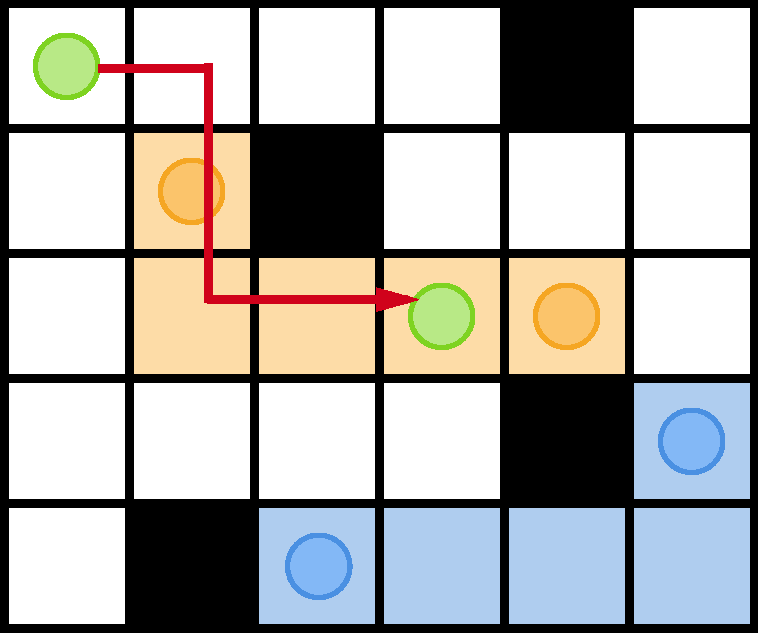
\includegraphics[width=.9\textwidth]{img/5-maze_update3}%
      \end{center}
    \end{column}
  \end{columns}
\end{frame}

\begin{frame}{Shared State Application: Labyrinth Benchmark}
  \begin{columns}
    \begin{column}{0.5\textwidth}
        \begin{block}{Amorphous Data Parallelism}
            behaviour observed in some irregular applications
        \end{block}

        \hfill

        \begin{itemize}
            % \item behaviour observed in some irregular applications\\ \ 
            \item<2-> processing one element may generate new work items or remove others
            \item<4-> some items cannot be processed in parallel due to conflicts
        \end{itemize}
    \end{column}
    \begin{column}{0.5\textwidth}
      \begin{center}
        \includegraphics<1-2>[width=.9\textwidth]{img/5-maze_update3}%
        \includegraphics<3->[width=.9\textwidth]{img/6-maze_update-noconflict}%
      \end{center}
    \end{column}
  \end{columns}
\end{frame}

\begin{frame}{Shared State Applications: Implementation}
    % TODO: Give that slide some love?
    \textbf{Problem:}\\
    \begin{itemize}
        \item Compiler analyses struggle to uncover meaningful parallelism
        \item<2-> Locking is too defensive
    \end{itemize}

    \vspace{1.5em}

    \uncover<3->{\textbf{Solution:} Optimistic Parallelism}
\end{frame}

\begin{frame}[t]{Optimistic Parallelism: Software Transactional Memory\footnotemark[1]}
    \centering%
    \includegraphics<1-2>[width=.8\textwidth,keepaspectratio]{img/background-stm1}%
    \includegraphics<3>[width=.8\textwidth,keepaspectratio]{img/background-stm2}%
    \includegraphics<4>[width=.8\textwidth,keepaspectratio]{img/background-stm3}%
    \includegraphics<5>[width=.8\textwidth,keepaspectratio]{img/background-stm4}%
    \includegraphics<6-10>[width=.8\textwidth,keepaspectratio]{img/background-stm5}%
    \includegraphics<11->[width=.8\textwidth,keepaspectratio]{img/background-stm_conf2}%
    \flushleft

    \begin{itemize}
        \only<1-7>{
            \item uses \emph{transactions} to guard access to shared data
            \begin{itemize}
                \item<2-> work similar to database transactions
                \item<7-> ensure atomicity, consistency and isolation
                % \item<4-> all changes within transaction take effect at once
            \end{itemize}
        }
        \only<8-9>{
            \item allows shared data access without blocking
            \item<9-> \textbf{optimistic:} assumes only few conflicts will happen
        }
        \only<10->{
            \item speculative parallelism leads to non-deterministic execution
        }
    \end{itemize}
    \footnotetext[1]{Shavit, et al. "Software transactional memory." Distributed Computing 10.2 (1997): 99-116.}
\end{frame}

\begin{frame}{Ohua\footnotemark[2]}
  \begin{columns}
    \begin{column}{0.7\textwidth}
      Framework for implicit parallel programming:\\[.55\baselineskip]
      \begin{itemize}
        \item<2-> Derives dataflow graph from algorithm file
        \item<3-> Runs optimizations on graph to exploit parallelism at compile time
        \item<4-> Generates native runtime code
        \item<5-> \textbf{Result:} Deterministic parallel program
      \end{itemize}
      % TODO: Zusätzlichen Punkt, der Ohua besser verkauft für dieses Problem.

      \vspace{1.5em}

      \uncover<5->{\emph{Is Ohua a possible alternative to STM?}}
    \end{column}
    \begin{column}{0.25\textwidth}
      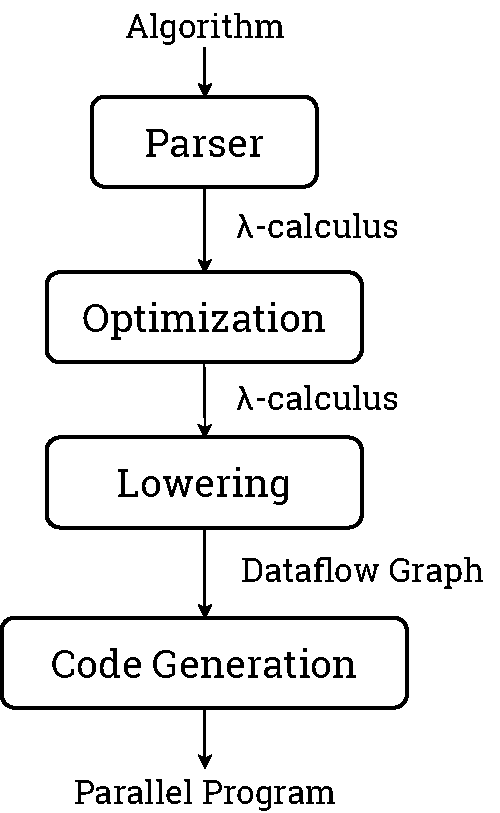
\includegraphics[width=\textwidth,height=\textheight,keepaspectratio]{img/ohua}
    \end{column}
  \end{columns}

  \footnotetext[2]{Ertel et al. "Towards Implicit Parallel Programming for Systems." dissertation, 2019.}
\end{frame}

\begin{frame}{Compiler Transformations}
    % TODO
\end{frame}

\begin{frame}{Performance Comparison}
    \begin{itemize}
        \item measured speedups for STM and Ohua
            \begin{itemize}
                \item<2-> 4 representative benchmarks from STAMP\footnote[3]{Minh, Chi Cao, et al. "STAMP: Stanford transactional applications for multi-processing." 2008 IEEE International Symposium on Workload Characterization. IEEE, 2008.} suite
                \item<3-> 3 different inputs\\ \ 
            \end{itemize}
        \item<4-> Result verification
            \begin{itemize}
                \item<4-> Compare STAMP (C) results with our STM performance (Rust)
                \item<5-> \textbf{Verification Criterion:} similar scaling behavior
            \end{itemize}
        \end{itemize}
\end{frame}

\begin{frame}{Results: Labyrinth}
    \begin{columns}%
        \begin{column}{0.5\textwidth}
            \centering
            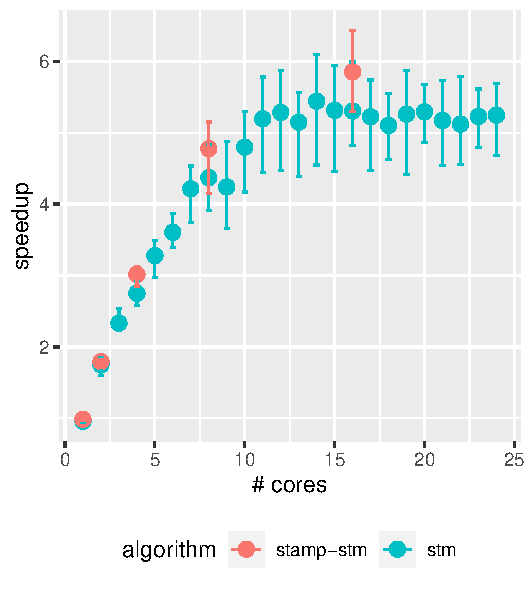
\includegraphics[width=\textwidth,height=.65\textheight,keepaspectratio]{img/combined_plots/labyrinth++}
        \end{column}%
        \begin{column}{0.5\textwidth}
            \begin{itemize}
                \item[\done]<2-> similar scaling behavior\\ \ 
                % \item TODO
            \end{itemize}
        \end{column}
    \end{columns}
\end{frame}

\begin{frame}{Results: Labyrinth}
    \begin{columns}%
        \begin{column}{0.5\textwidth}
            \centering
            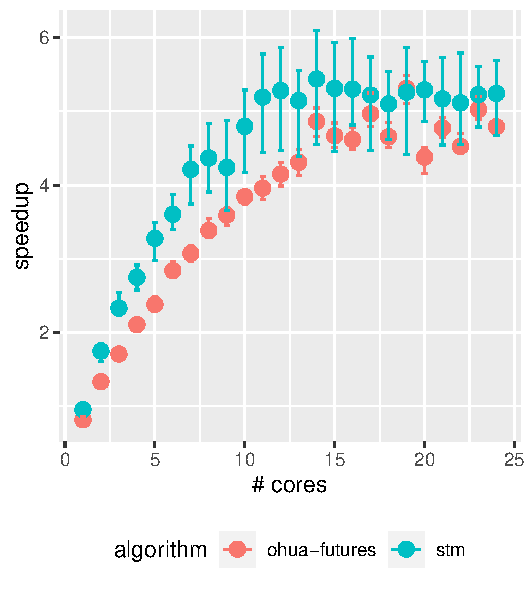
\includegraphics[width=\textwidth,height=.65\textheight,keepaspectratio]{img/results/labyrinth++}
        \end{column}%
        \begin{column}{0.5\textwidth}
            \begin{itemize}
                \item<2-> Ohua almost on par with STM
                \begin{itemize}
                    \item<3-> less variance in measured values\\ \ 
                \end{itemize}
                \item<4-> STM: non-deterministic
                \begin{itemize}
                    \item<5-> varying number of conflicts
                \end{itemize}
            \end{itemize}
        \end{column}
    \end{columns}
\end{frame}

\begin{frame}{Results: Intruder}
    \begin{columns}%
        \begin{column}{0.5\textwidth}
            \centering
            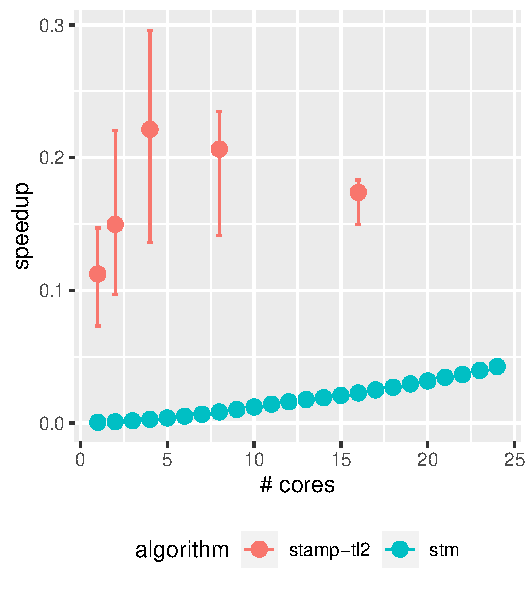
\includegraphics[width=\textwidth,height=.65\textheight,keepaspectratio]{img/combined_plots/intruder+}
        \end{column}%
        \begin{column}{0.5\textwidth}
            \begin{itemize}
                \item[\nope]<2-> worse scaling behavior\\ \
            \end{itemize}

            \uncover<3->{\textbf{Possible Reasons:}}
            \begin{itemize}
                \item<3-> STAMP is heavily optimized \\ (e.g., own HashMap)
                \item<4-> tried to replicate this in Rust
                % TODO fix this
            \end{itemize}
        \end{column}
    \end{columns}
\end{frame}

\begin{frame}{Results: k-means (low contention)}
    \begin{columns}%
        \begin{column}{0.5\textwidth}
            \centering
            \includegraphics<-6>[width=\textwidth,height=.65\textheight,keepaspectratio]{img/combined_plots/kmeans-low++}%
            %\includegraphics<7->[width=\textwidth,height=.65\textheight,keepaspectratio]{img/combined_plots/kmeans-low++}%
            % TODO: Show CPU use?
        \end{column}%
        \begin{column}{0.5\textwidth}
            \begin{itemize}
                \item[\done]<2-> nearly similar scaling behavior\\ \ 
            \end{itemize}

            %\uncover<3->{\textbf{Possible Reasons:}}
            \begin{itemize}
                \item<3-> performance drop for large thread counts
                \item<4-> \textbf{Reason:} differences in memory sharing
                \begin{itemize}
                    \item<5-> C version uses single copy of data structure
                    \item<6-> Rust must create copies of data for each thread
                \end{itemize}
            \end{itemize}
        \end{column}
    \end{columns}
\end{frame}

\begin{frame}{Results: k-means (low contention)}
    \begin{columns}%
        \begin{column}{0.5\textwidth}
            \centering
            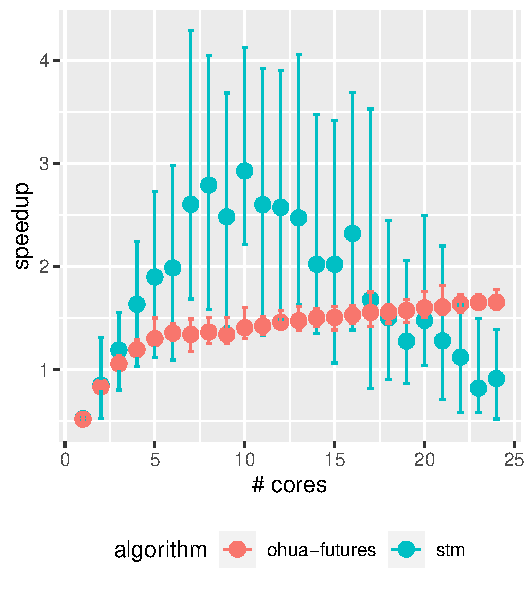
\includegraphics[width=\textwidth,height=.65\textheight,keepaspectratio]{img/results/kmeans-low++}%
        \end{column}%
        \begin{column}{0.5\textwidth}
            \begin{itemize}
                \item TODO
            \end{itemize}
        \end{column}
    \end{columns}
\end{frame}

\begin{frame}{Results: k-means (high contention)}
    \begin{columns}%
        \begin{column}{0.5\textwidth}
            \centering
            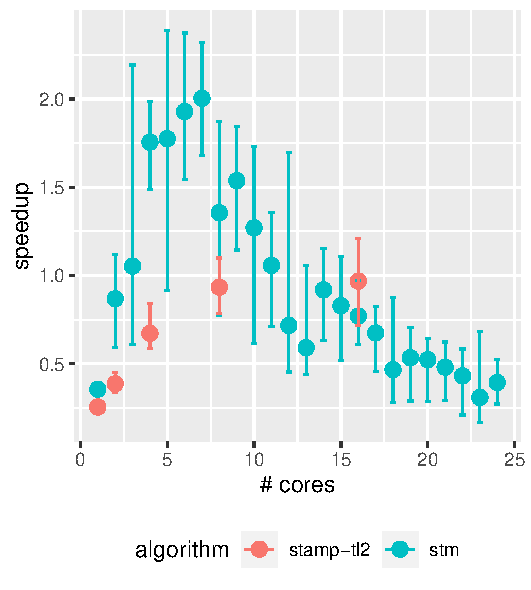
\includegraphics[width=\textwidth,height=.65\textheight,keepaspectratio]{img/combined_plots/kmeans-high++}
        \end{column}%
        \begin{column}{0.5\textwidth}
            \begin{itemize}
                \item[\done]<2-> Rust version outperforms STAMP\\ \ 
            \end{itemize}
            
            \begin{itemize}
                \item<3-> same behavior as in low contention run
            \end{itemize}
        \end{column}
    \end{columns}
\end{frame}

\begin{frame}{Results: k-means (high contention)}
    \begin{columns}%
        \begin{column}{0.5\textwidth}
            \centering
            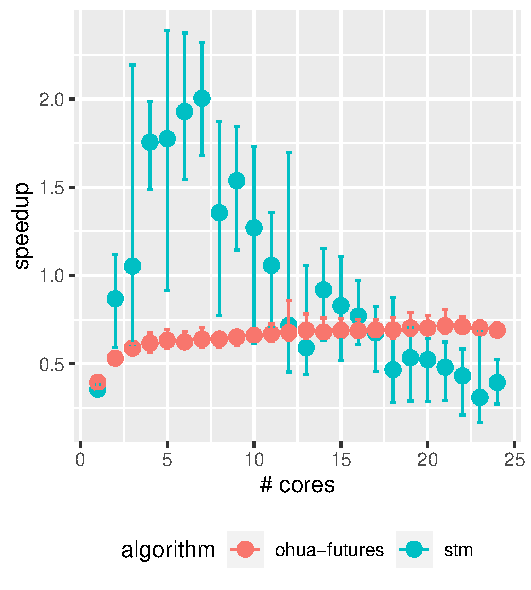
\includegraphics[width=\textwidth,height=.65\textheight,keepaspectratio]{img/results/kmeans-high++}
        \end{column}%
        \begin{column}{0.5\textwidth}
            \begin{itemize}
                \item TODO
            \end{itemize}
        \end{column}
    \end{columns}
\end{frame}

\begin{frame}{Results: Genome}
    \begin{columns}%
        \begin{column}{0.5\textwidth}
            \centering
            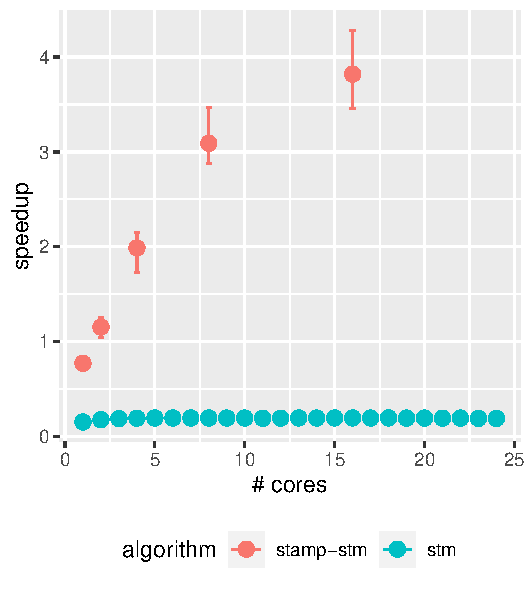
\includegraphics[width=\textwidth,height=.65\textheight,keepaspectratio]{img/combined_plots/genome++}
        \end{column}%
        \begin{column}{0.5\textwidth}
            \begin{itemize}
                \item[\nope]<2-> completely different curve shapes\\ \ 
            \end{itemize}

            \uncover<3->{\textbf{Possible Reasons:}}
            \begin{itemize}
                \item<3-> STAMP is more optimized \\ (e.g., own HashSet)
                \item<4-> high overhead for data duplication (24 \% of total time used)
            \end{itemize}
        \end{column}
    \end{columns}
\end{frame}

\begin{frame}{Results: Remarks}
    \begin{itemize}
        \item Transformations 2 \& 3 proved useful for parallelization
        \begin{itemize}
            \item<2-> used for \texttt{labyrinth}
            \item<3-> only applicable for amorphous data parallel applications\\ \
        \end{itemize}
        \item<4-> optimizing other irregular applications requires deeper insight into shared state usage
        \begin{itemize}
            \item<5-> workset partitioning could be used to parallelize state loops
        \end{itemize}
    \end{itemize}

    \uncover<6->{
    \begin{block}{Research Question}
        How can we better understand workset partitionability to exploit this?
    \end{block}}
\end{frame}

\begin{frame}{Conclusions}
    \textbf{Could Ohua be an alternative to STM for shared state applications?}

    \vspace{1.5em}

    \begin{itemize}
        \item<2-> yes, for \emph{some} applications
        \item<3-> further research into state partitioning necessary to exploit other applications
    \end{itemize}
\end{frame}

\begin{frame}
  \centering
  \huge
  \alert{\textbf{Thank you for your attention.}}
\end{frame}

% -----------------------------------------------------------------------------------------------------------
% ---------------------------------------------- BACKUP Slides ----------------------------------------------
% -----------------------------------------------------------------------------------------------------------

\begin{frame}
  \centering
  \huge
  \alert{\textbf{Backup}}
\end{frame}

\begin{frame}{Backup: Representative Benchmark Selection}
    \centering
    \begin{tabular}{|l|l|l|l|l|l|}
        \hline
        \textbf{Application} & \textbf{tx length} & \textbf{r/w set} & \textbf{tx time} & \textbf{Contention}\\\hline\hline
        labyrinth & long & large & high & high\\\hline
        bayes & long & large & high & high\\\hline
        yada & long & large & high & medium\\\hline
        vacation & medium & medium & high & low/medium\\\hline
        genome & medium & medium & high & low\\\hline
        intruder & short & medium & medium & high\\\hline
        kmeans & short & small & low & low\\\hline
        ssca2 & short & small & low & low\\\hline
    \end{tabular}
\end{frame}

\begin{frame}[fragile]{Backup: Differences in Memory Sharing}
    \begin{minted}[bgcolor=rustcolor]{C}
        unsigned long data[] = {1, 2, 3, 4, 5, 6, 7, 8, 9, 10};

        pid_t pid = fork();
        if (pid != 0) {
            int lower = 0;
            int upper = 4;
            // changes elements at indices 0 to 4
            modify_elements(data, lower, upper);
        } else {
            int lower = 5;
            int upper = 9;
            // changes elements at indices 5 to 9
            modify_elements(data, lower, upper);
        }
    \end{minted}

    %\begin{itemize}
        %\item impossible to do in Rust
    %\end{itemize}
\end{frame}

\end{document}
